%%%%%%%%%%%%%%%%%%%%%%%%%%%%%%%%%%%%%%%%%%%%%%%%%%%%%%%%%%%%%%%%%%%%%%%%%%%%%%%
% Chapter 4 : Desarrollo de la Aplicación
%%%%%%%%%%%%%%%%%%%%%%%%%%%%%%%%%%%%%%%%%%%%%%%%%%%%%%%%%%%%%%%%%%%%%%%%%%%%%%%

%++++++++++++++++++++++++++++++++++++++++++++++++++++++++++++++++++++++++++++++

En el capitulo ~\ref{chapter:tres} se describieron las funcionalidades de la aplicación. A continuación
hablaremos de todo lo que conllevó el proceso de  elaboración del proyeto, desde su comienzo hasta el final,
incluyendo las entrevistas, problemas, etc.


%++++++++++++++++++++++++++++++++++++++++++++++++++++++++++++++++++++++++++++++

\section{Primeros Pasos}
\label{4:sec1}

Partimos de una implementación en PHP, que poseía las funcionalidades básicas, pero el problema era que la base de datos
no era compatible con nuestra tecnología, debido a que seguía el modelo entidad-relación, y nosotros al contrario, necesitábamos
crear una base de datos no relacional. Por otro lado teníamos de ejemplo la aplicación web ``online scout'', la cual era muy completa
pero era de pago, y nuestro objetivo era hacer una aplicación gratuita adaptada al cliente, en nuestro caso la organización de scout Aguere 70 de La Laguna.\\

Para adaptarla lo mejor posible, lo primero que hicimos fue tener una reunión con el grupo scout Aguere 70, previamente a esta reunión se realizó una serie de tutoriales
básicos de Django para refrescar conocimientos, ademas de hacer pruebas con la tecnologia de Google App Engine e incorporarlas al framework de django-nonrel.\\ 

Después de estos pasos previos, se realizo la primera reunión con el grupo Aguere 70, en la que se elaboró un análisis de requisitos, se estudiaron las posibles 
funcionalidades que tendría la aplicación, seleccionando las funciones fundamentales, debido al corto tiempo y personal que había para realizar la aplicación.\\

\section{Requisitos Iniciales}
\label{4:sec2}

Después de la reunión con los interesados se estableció un esquema compuesto por 7 aplicaciones,
la cual una de ellas era la principal y de esa dependerían el resto. Las aplicaciones son las siguientes:
\begin{itemize}
\item Socios: esta es la aplicación principal que tendrá los datos de los socios que usaran las demás aplicaciones. Contiene:
	\begin{itemize}
	\item Mantenimiento de socios
	\item Cambios de Unidad
	\item Informes (Familiares, Unidades, Médicos, Personales)
	\item Exportaciones
	\end{itemize}

\item Lista de espera
	\begin{itemize}
	\item Entradas
	\item Propuestas de entrada a grupo
	\item Incidencias
	\end{itemize}

\item Biblioteca
	\begin{itemize}
	\item Mantenimiento
	\item Préstamos
	\end{itemize}

\item Intendencia
	\begin{itemize}
	\item Mantenimiento
	\item Préstamos
	\item Informes
		\begin{itemize}
		\item Prestados
		\item Estados
		\end{itemize}
	\item Campamentos
	\end{itemize}
\item Recursos
	\begin{itemize}
	\item Dinámicas
	\item Talleres
	\item Juegos
	\item Resto de Actividades
	\end{itemize}

\item Tesorería
	\begin{itemize}
	\item Control de Cuentas
	\item Presupuestos
	\item Emisión de recursos
	\item Resúmenes
		\begin{itemize}
		\item Anual
		\item Trimestral
		\end{itemize}
	\end{itemize}

\item Varios
	\begin{itemize}
	\item Compañía de seguridad
	\item Agenda
	\item Recetario
	\end{itemize}
\end{itemize}

Visto las siguientes aplicaciones se comprobó que el proyecto era ambicioso y extenso, 
por lo tanto nos enfocamos en el apartado de la app de Socios que era la mas importante. 
Se nos facilitó la ficha de inscripción en formato papel que han de cumplimentar los socios para inscribirse en la organización.
Por tanto nos sirvió de modelo para generar una primera aproximación del modelo de datos que va a llevar la aplicación de Socios.\\

[[Espacio para el primer modelo de datos]]

\section{Preparación para el proyecto}
\label{4:sec3}

Primero que nada necesitamos instalar el framework de django-nonrel, para ello lo que se hizo fue crear un nuevo proyecto vacío con el 
programa ``Aptana Studio 3'', el cual debía de tener los archivos que nos proporciona la web ``www.allbuttonspressed.com'' que contienen 
todos los archivos necesarios para configurar un proyecto que funcione con django-nonrel y Google App Engine, 
de modo que el proyecto nos quedaría de la siguiente manera:

\begin{itemize}
  \item \lstinline!django-nonrel/django => <project>/django!
  \item \lstinline!djangotoolbox/djangotoolbox => <project>/djangotoolbox!
  \item \lstinline!django-autoload/autoload => <project>/autoload!
  \item \lstinline!django-dbindexer/dbindexer => <project>/dbindexer!
  \item \lstinline!djangoappengine => <project>/djangoappengine!
\end{itemize}

\textbf{Importante:} Al instalar el SDK de App Engine incluir el PATH en el archivo .profile de nuestra carpeta personal en Linux.\\

Por otro lado es importante hablar del archivo de configuración app.yaml, que especifica la manera en la que las rutas de URL se corresponden con los 
controladores de solicitudes y con los archivos estáticos en el entorno de Google App Engine. 
También debe contener información sobre el código de la aplicación como, por ejemplo, el ID de la aplicación y el identificador de la última versión.\\

De modo que el arhivo seria el siguiente:\\
\lstinputlisting[caption={Archivo de configuración app.yaml}]{codes/app.yaml}


\section{Inicio de sesión}
\label{4:sec4}

Como se ha dicho en el capitulo ~\ref{chapter:tres} el inicio de sesión esta limitado al dominio del grupo de scout de Aguere 70, lo cual se accede a la aplicación
por medio de sus cuentas de google asociadas a dicho dominio.\\

El archivo settings.py se configuró de la siguiente manera:\\

\lstinputlisting[caption={Ejemplo de listado desde archivo}]{codes/authentication_settings.py}




Donde se puede apreciar las \textsc{INSTALLED APPS} necesarias para este apartado de la aplicación. Pasamos a describir cada una:\\
\begin{itemize}
\item \textbf{djangoappengine}: es un backend para poder utilizar la base de datos que nos brinda Google App Engine.\\

\item \textbf{gaeauth}: es otro backend que nos facilita el inicio de sesión a traves de la interfaz de Google Accounts, 
para iniciar sesión con las cuentas de Google en nuestra aplicación.\\

Es la ultima parte del archivo settings.py se ve claramente que esta seleccionado en \textsc{AUTHENTICATION BACKENDS} el backend de gaeauth y seguidamente elegimos en \textsc{ALLOWED DOMAINS} el dominio
en el cual queremos restrigir el acceso, en nuestro caso solo los usuarios pertenecientes al dominio ``gruposcoutaguere70.org'' podran acceder a la aplicación.

\item \textbf{plus}: Este es el modulo que nos permite obtener la información personal, foto de perfil y demás datos de los usuarios que acceden a la aplicación por medio de su cuenta de Google+, sin necesidad
de guardar esos datos en nuestra base de datos.

Este fue uno de los modulos que más dio problemas. Primero habia que acceder a la web de Google APIs con la cuenta de desarrollador y activar la API de Google+ posteriormente tenemos que editar el acceso a las APIs,
para introducir nuestra aplicación en el entorno, por lo tanto se nos generaria una serie de datos que podriamos introducirlos en nuestra aplicación uno a uno o bien en formato JSON, este paso es importante ya que sino la aplicación
no podría acceder a los servicios que nos proporciona la API.

Dicho esto una vez que el usuario inicia sesión, en el proceso se accede a la vista de la app plus, que esta cargara la configuración de Google API por medio del mencionado archivo JSON o introduciendo una a una 
de la siguiente manera la configuración necesaria para utilizar el servicio de Google+:\\

\lstinputlisting[caption={Ejemplo de listado desde archivo}]{codes/flow_plus.py}

Donde \textbf{client-id} y \textbf{client-secret} son los datos que apuntan al acceso de API que ha establecido el programador de la aplicación, \textbf{token-uri} lo delegamos para que lo ejecute oauth2, en \textbf{scope}
se añaden las direcciones de las API que se van a usar, en nuestro caso la de Google+ y la de Drive(esta la explicaremos mas adelante), en \textbf{redirect-uri} establecemos la direccion de retorno a nuestra aplicación 
por medio de la llamada oauth2cabllback que la incorpora el modulo plus.

Con todo esto lo que logramos es que en el inicio de sesión se establezca una conexion entre el usuario y las APIs de google, en la cual se acepten una serie de permisos para posteriormente generar una credencial,
que se guardará en el usuario, con la cual podra acceder a los servicios activados previamente por el programador en Google APIs. Es importante señalar que el modelo de User que nos ofrece django se modificó para que
se pudieran guardar las credenciales, ademas se añadio el campo de \textbf{cargo}, donde se le asignara a cada usuario un cargo especifico, por tanto las funciones que podra realizar en la aplicación estaran supeditadas a dicho cargo.

\textbf{Nota:} las credenciales suelen expirar a la hora por tanto, una vez expiradas el usuario no podra acceder a la aplicación, al menos que se actualicen. Una forma de automatizar esto es que en cada inicio de sesión
se restablescan las credenciales, por eso añadimos dos campos mas a la variable FLOW, que son el \textbf{access-type='offline'} y \textbf{approval-prompt='force'} con esto logramos forzar el refrezco de
credenciales una vez estas caduquen.
\end{itemize}

\section{Creación de Usuarios}
\label{4:sec5}

Una vez definida la primera aproximación del modelo de datos que vamos a emplear en la aplicación, empezamos con la creacion de la app de socios que va a gestionar todo lo referente a la información de los socios de 
la organización.\\

Esta tarea era simple pero tediosa a la hora de realizar templates, formularios, etc, para que luego en la vista de la app de socios por medio de diferentes llamadas POST, se fueran contruyendo los objetos necesarios
para la creacion de un nuevo socio, cada objeto almacenaba un tipo de información especifica segun el modelo de datos. Por tanto el modelo final de socios tenia las siguientes tablas:\\

\lstinputlisting[caption={Ejemplo de listado desde archivo}]{codes/model_socio.py}

Como podemos ver el modelo esta compuesto por 8 tablas, debido a que no se pueden establecer relaciones en la base de datos de tipo no relacional, la unica forma de en cierto modo comunicar/unir una tabla con otra,
es con lo que llamamos claves foraneas(ForeignKey), de esta manera podremos asosciar las tablas que nos interesen de manera unidimensional.\\

Se puede observar para que es cada tabla y el tipo de información que guarda, se dejo elaborada aunque no se usa todavía la tabla de \textbf{Autorizasiones} para que en un futuro los socios almacenen ahí las posibles autorizaciones/permisos
cuando se realice una excursión, uso de fotografias de manera pública, etc.\\

Retomando a la creación de usuarios es necesario rellenar todos los campos importantes de cada objecto para conservar la integridad de la base datos. Los formularios comprueban que esto se cumpla y al finalizar lo manda como un POST
al servidor donde es procesado y si todo esta correcto se guarda en la base de datos.\\

Por otro lado en la carpeta \textbf{templates/socios} están todos los archivos .html que se usan para la interacción del usuario desde el cliente con el servidor, las template que se usan para la creación de usuario se distinguen por 
empezar por \textbf{f-[nombreTabla].html}


\section{Modificación de Usuarios}
\label{4:sec6}
Un proceso similar al de creación de usuarios se implementó para la modificación de los respectivos datos de los socios, los archivos de las templates eran similares, salvo que tienen trozos de código en Javascript
y variables que se pasaban de la vista a la template para autocompletar los campos de los formularios con los datos del socio, de esta forma si se va a editar un campo en concreto no es necesario rellenar 
todos los campos restantes.\\

Los archivos de templates relacionados con la edición de datos de los usuarios se caracterizan por tener la siguiente nomenclatura \textbf{f-edit-[nombreTabla]}
\section{Listados de información}
\label{4:sec7}
Se implementaron dos formas de visualizar los datos de los socios, la mas simple es una vez obtenido el ID del socio, se accede a las paginas de información del socio, donde cada template esta enfocada a una determinada tabla
del modelo de datos, de esta forma los datos los clasificariamos en personales, economicos, medicos y familiares. En la vista lo unico que se hace es volcar los datos del socio a la template, que es la que se encarga de 
la visualización de los repectivos datos.

\lstinputlisting[caption={Ejemplo de listado desde archivo}]{codes/datos_economicos.py}

Por otro lado para tener un vistazo general de los socios, se elaboró una tabla donde se listan todos los socios mostrando sus datos acorde con el listado en el que se este, es decir existen varios listados para representar los 
datos de los socios, listados de datos personales, economicos, etc.\\

Para el formato de la tabla se encontro un widget con la  apariencia de bootstrap para mantener la escencia de la interfaz visual, en cuyas tablas se pueden
realizar ordenaciones, filtrados y exportaciones que describirán detalladamente en los siguientes apartados.

\section{Filtrado de tablas}
\label{4:sec8}
Para poder utilizar las funciones de filtrado y ordenaciones en los listados, era necesario incorporar en nuestra aplicación los siguientes scripts:\\

\lstinputlisting[language=html,basicstyle=\scriptsize,caption={Ejemplo de listado desde archivo}]{codes/script_tablesorter.html}

En la zona comentada de cada script se nombra para que se utiliza cada uno. Ademas de estos script es necesario introducir una función en Javascript que nos  proporciona el propio widget donde se especifican la configuracion de 
tabla, como el tema de apariencia, los filtros, paginación etc.\\

Posteriormente la estructura de la tabla lleva la siguiente sintaxis:\\

\lstinputlisting[language=html,caption={Ejemplo de listado desde archivo}]{codes/sintaxis_tabla.html}

\section{Exportaciones a Google Drive}
\label{4:sec9}

Para poder llevar las exportaciones a Google Drive primero que nada se tiene que establecer un permiso entre el  usuario, la aplicación y la API de Google Drive para poder utilizar el servicio. Esto con las credenciales que se han
comentado en la sección de \textbf{Inicio de Sesión}, añadiendo en el campo de \textbf{scope} la ruta al servicio Drive antes de generar la credencial.\\

Ahora bien, los filtrados de los listados se realizan sobre la template en el cliente, por tanto si quieremos exportar una listado filtrado tenermos que en cierto modo, realizar el filtrado en el lado del servidor.
Esto se logro modificando los archivos del \textbf{tablesorter} para que cuando generara la tabla, cada input de filtrado tenga un nombre (\textbf{name}), el cual se utiliza cuando se realiza una llamada POST, para poder obtener los parametros de filtrado.
y realizar el filtrado directamente con el modelo de datos.\\

Una vez realizado esto, nos queda el paso intermedio para poder exportar los datos a Google Drive, ya que para exportar necesitamos crear un fichero de extensión .csv para que la API de Google Drive lo interprete y lo procese.
De modo que la construcción del fichero se realizó de la siguiente manera:\\

\lstinputlisting[caption={Ejemplo de listado desde archivo}]{codes/export_drive.py}

\section{Cambios de Unidad}
\label{4:sec10}

Esta función fue bastante demandada por la organización y consiste en crear una función que calcule la edad de los socios y en según la edad los clasifique en la sección/unidad que le corresponda de acuerdo al rango previamente
establecido.\\

El código de dicha función es el siguiente:\\

\lstinputlisting[caption={Ejemplo de listado desde archivo}]{codes/cambio_unidad.py}

\section{Importación de base de datos antigua}
\label{4:sec11}

La organización de scout Aguere 70 tiene una base de datos donde hasta el momento guarda los datos de los socios, todos los datos están almacenados en una sola tabla y se nos propuso si era posible importar esta base de datos
y volcarla en nuestra aplicación.\\

El principal problema era que esta toda la información en un sola tabla por tanto habria que implementar un mecanismo para separar la información y adaptarla a nuestro modelo de datos.\\

Por otro lado tenemos el formato del fichero de la base de datos que estaba en formato \textbf{Access}, de modo que era necesario convertirlo a un formato que pudiera procesar la aplicación de manera eficiente. Se pensó 
en el formato .csv separado por comas, ya que habia una herramienta llamada \textbf{MDB Tools} que convertia los ficheros accecc en csv.

Una vez obtenido el fichero csv, se implemento un mecanismo para subir el fichero a la aplicación sin que este se guardara en el servidor, sino que solo estuviera ahí mientras se este procesando. De modo que se creo 
una nueva app llamada \textbf{upload} especificamente para este proceso.\\

Esta app tiene un fichero \textbf{forms.py} que contiene el formato del form para datos de tipo fichero (FileField).\\

\lstinputlisting[caption={Ejemplo de listado desde archivo}]{codes/form_upload.py}
\bigskip
Esto lo procesa la template y posteriormente con la llamada de POST se envia el archivo al servidor, que se tratara de la manera siguiente:
\bigskip
\lstinputlisting[caption={Ejemplo de listado desde archivo}]{codes/transformacion_fichero.py}

Después se procesa casilla a casilla el array y se introducen los datos en la base de datos, siempre cuidando la integridad de la base de datos, de modo que no queden ambiguedades, ni campos vacios que sean importantes 
en cada tabla del modelo.\\

\section{Calidad de Código: Pylint}
\label{4:sec12}
Para finalizar el periodo de desarrollo del proyecto, mejoramos la calidad de código de los principales archivos escritos en Python de la aplicación. Para ello utilizamos la herramienta Pylint, obteniendo una nota media en los
archivos de 9.0 en cuanto a calidad de código.\\


\begin{figure}[H]
\begin{center}
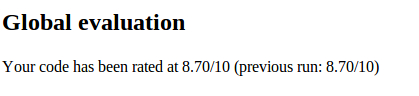
\includegraphics[width=0.75\textwidth]{images/pylint.jpg}
\caption{Resultado tras analizar socios/views.py con el Pylint.}
\label{fig:ArbolBinario}
\end{center}
\end{figure}








